\section{Zielsetzung}
Das Ziel der Arbeit ist es, eine konkrete Programmiersprache anhand von einigen Vorgaben zu definieren. Die neue Programmiersprache soll sich stark an den beiden Programmiersprachen \enquote{loop} und \enquote{while}, welche im neunten Kapitel im Buch \citetitle{GottfriedVossen2016} von \citeauthor{GottfriedVossen2016} beschrieben werden, orientieren. \cite{GottfriedVossen2016} Es müssen sich Gedanken gemacht werden, wie Konzepte aus dem Buch in einer tatsächlichen Programmiersprache syntaktisch umgesetzt werden und inwiefern die Sprache sinnvoll erweitert werden kann, ohne den Grundgedanken der Sprachen aus den Augen zu verlieren.



\begin{figure}[h!]
	%\includegraphics[width=1\textwidth]{content/pictures/LoRaWAN-OSI.JPG}
	\centering
	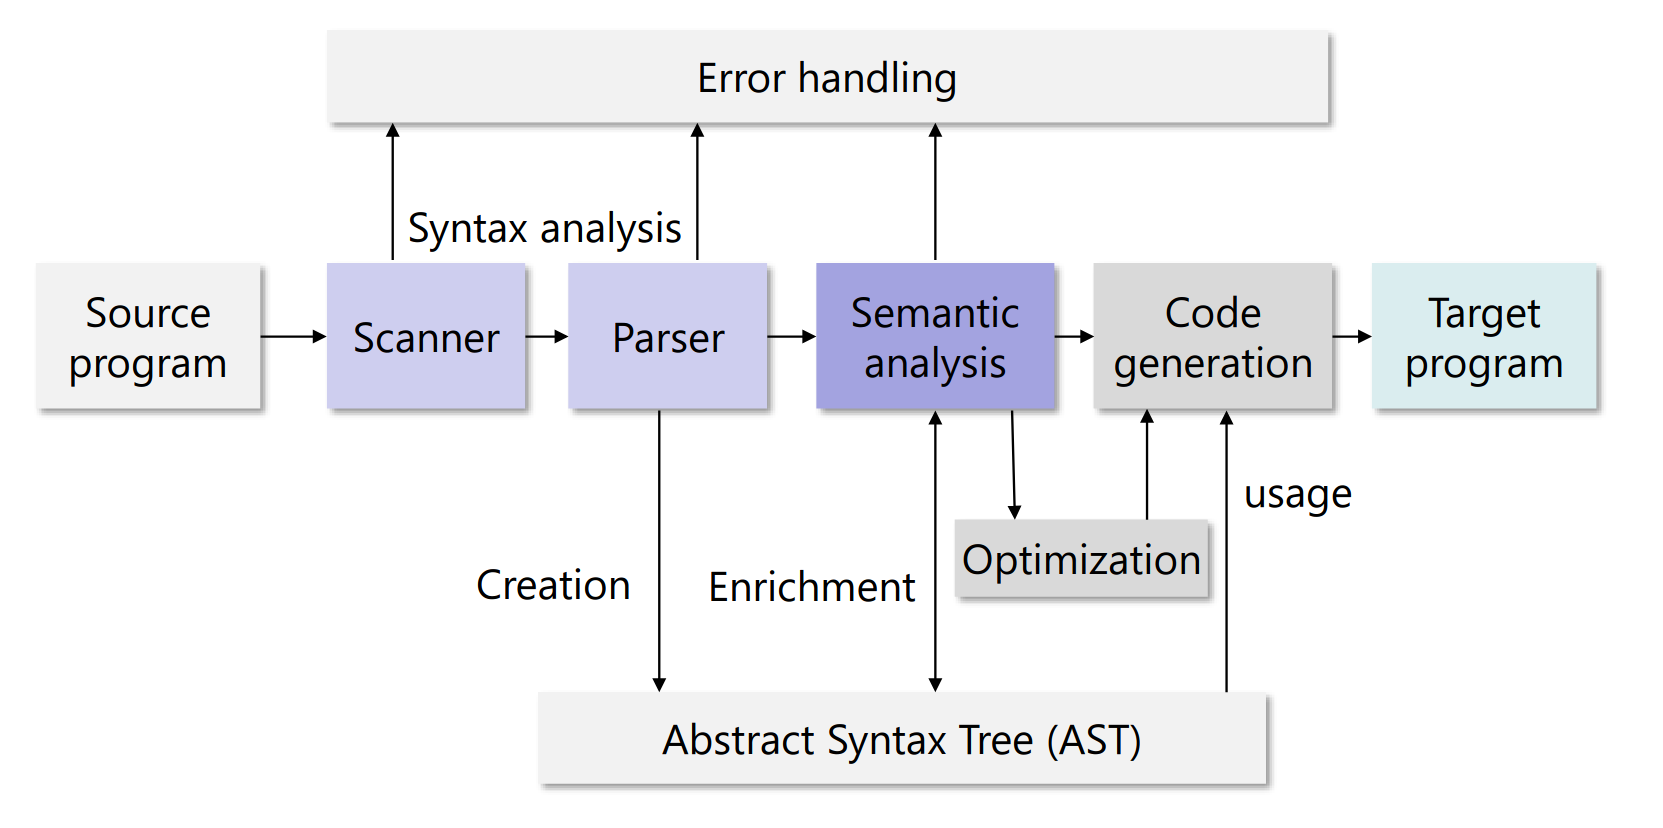
\includegraphics[width=12cm]{content/pictures/compiler.png}
	\captionsource{Aufbau eines Compilers}{\cite{BernhardHollunder2022}}
	%	\source{\cite[S. 5]{SemtechCorporation.2020}}
	\label{pic:CompilerAufbau}
\end{figure}

Anschließend soll ein Compiler für die definierte Sprache entwickelt werden. Dieser Compiler muss in der Lage sein, ein vom Benutzer geschriebenen Programmcode auf Fehler zu prüfen, gegebenenfalls Fehler auszugeben und letztendlich eine ausführbare Datei für die \ac{jvm} zu erzeugen. In der \cref{pic:CompilerAufbau} ist der grundlegende Aufbau eines Compilers zu sehen und damit die einzelnen Bestandteile, welche umgesetzt werden müssen.

Anschließend soll für die entwickelte Programmiersprache eine IDE-Integration erfolgen, um den Nutzer bei der Entwicklung von Programmen mit Features wie Syntax-Highlight zu unterstützen.